% Preamble
\documentclass[a4paper, 12pt]{article}
\usepackage[margin=1in]{geometry} % Set margin
\usepackage{pdfpages} % Insert pdf pages
\usepackage{amssymb,amsmath,amsthm, amsfonts} % Math libraries

% Custom commands
\newcommand{\sub}[1]{\subsection{\underline{#1}}}
\newcommand{\subsub}[1]{\subsubsection{\underline{#1}}}
\newcommand{\R}{\ensuremath{\mathbb{R}}}
\newcommand{\F}{\ensuremath{\mathbb{F}}}
\newcommand{\N}{\ensuremath{\mathbb{N}}}
\newcommand{\Onef}{\ensuremath{1_{\F}}}
\newcommand{\Zerof}{\ensuremath{0_{\F}}}
\newcommand{\eqbcuz}[1]{\text{~$\stackrel{(#1)}{=}$~}}
\newcommand{\eq}[1]{\begin{align*}#1\end{align*}}
\newcommand{\eqn}[1]{\begin{align}#1\end{align}}
\renewcommand{\qed}{\hfill\(\qedsymbol\)}
\newtheorem{lemma}{Lemma}

% Begin Document %
\begin{document}

% Title Page
\begin{titlepage}
    %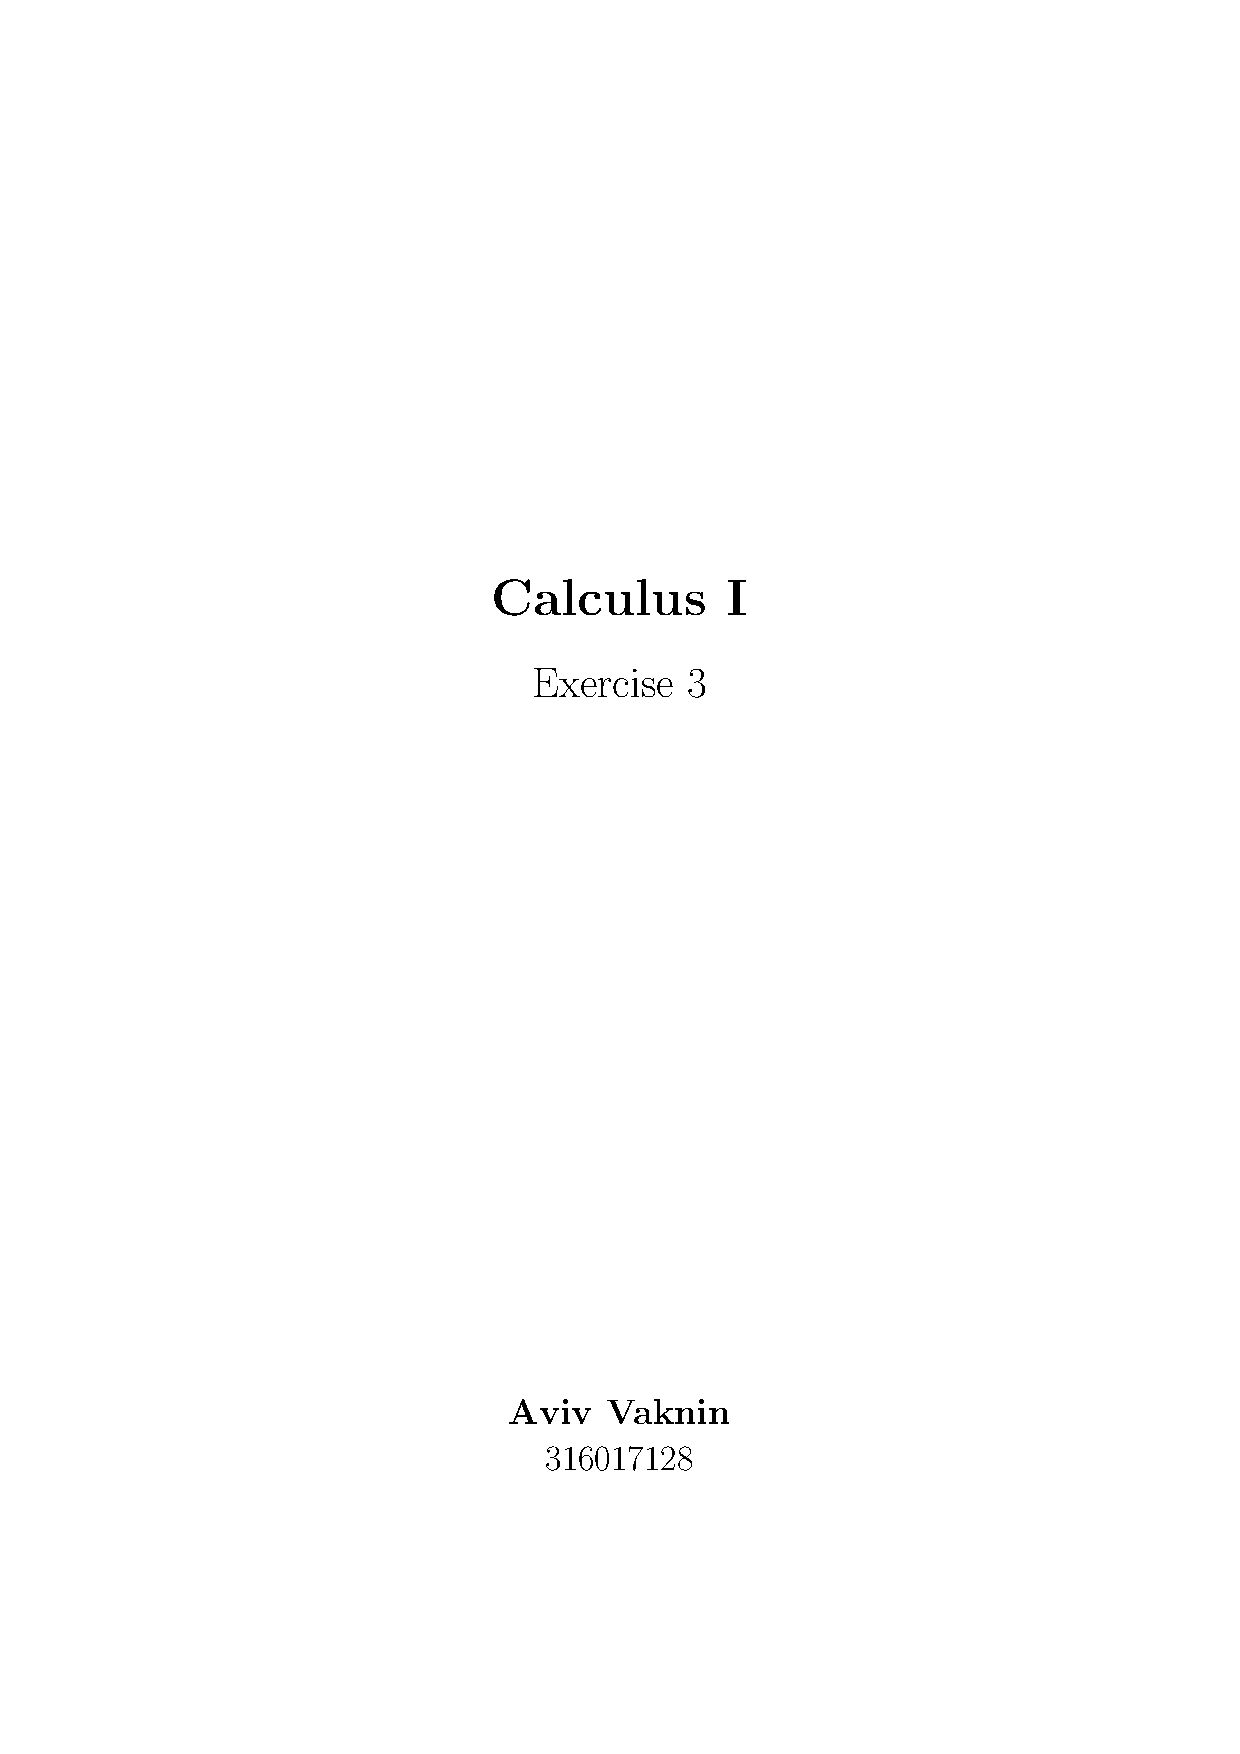
\includepdf{title.pdf}
\end{titlepage}

%1
\section{
$A\subseteq\F$, prove $m\in\F$ is the infimum of A \underline{\textit{if and only if}}:}
\begin{enumerate}
    \item m is the lower bound of $A$
    \item $(\forall\epsilon>0)~(\exists{a}\in{A})~(a<m+\epsilon)$
\end{enumerate}
\sub{$\implies$:}
We'll start with assuming $m\in\F$ is the infimum of $A$.\\
By definition, the infimum is a lower bound \textbf{(1)}.\\
Therefore: \eq{\forall{a}\in{A}~~a\geq{m}}
and, suppose $m'$ is another lower bound for $A$: \eq{m\geq{m'}}
First, by definition, an infimum is a lower bound.\\
Regarding the second item, let's suppose by contradiction:
\eq{\exists\epsilon>0~~\forall{a}\in{A}~~a\geq{m+\epsilon}\\m+\epsilon>m}
Therefore, we can see that $\underline{m+\epsilon}$ is a lower bound for $A$, bigger than the infimum.\\
We've reached a contradiction, as we've assumed $m$ is the infimum of $A$ \textbf{(2)}.
\sub{$\impliedby$:}
Let's suppose that $m$ is not the infimum.\\
Therefore, exists another lower-bound - $m'$ so that $m'>m$.\\
Let $\epsilon>0$: \eq{\epsilon=m'-m\\m'=\epsilon+m}
Therefore: \eq{\forall\epsilon>0~~\exists{a}\in{A}~~a\geq\epsilon+m}
Which is in contradiction with our initial assumption: \eq{(\forall\epsilon>0)~(\exists{a}\in{A})~(a<m+\epsilon)}
\qed\pagebreak

%2
\section{\eq{A\subseteq\F\\s\in\F}}
\sub{Prove $s=\max(A) \iff (s=\sup(A)) \land (s\in{A})$}
\subsub{$\implies$:}
Let's start by supposing $s=\max(A)$.\\
By definition, the maximum is always part of the set, therefore \textbf{(1)}: \eq{s\in{A}}
Let's show that $\max(A)=\sup(A)$:\\
We know from definition, that \textit{s} is an upper-bound of $A$.\\
Let's take any arbitrary $\epsilon>0$, therefore because $s\in{A}$:
\eq{s>s-\epsilon}
Therefore, by the definition of the supremum(proposition 5.7 in class), $s$ is $A$'s supremum.\textbf{(2)}
\subsub{$\impliedby$:}
Let's suppose that $s=\sup(A)$ and $s\in{A}$.\\
According to the definition of the maximum, if $s$ is the maximum of $A$, it must be:
\begin{enumerate}
    \item a member of $A$
    \item a supremum of $A$
\end{enumerate}
Both are given.
\qed
\sub{Prove that if $A$ has a maximum, there's only one.}
By definition, if a set has a maximum, it fulfills the following properties:
\begin{enumerate}
    \item it is a member of the set
    \item it is a supremum of the set
\end{enumerate}
Suppose $m$ is the maximum of $A$.\\
By definition, it must be part of $A$, satisfying \textbf{(1)}.
Because of \textbf{(2)}, it must be a supremum.
\subsub{n's smaller than m}
According to the definition of the upper-bound: \eq{\forall{\epsilon}>0~~\exists{a}\in{A}~~a>m-\epsilon}
Therefore, $m-\epsilon$ is smaller than $m$, and is not an upper-bound, therefore not a maxmium.
\subsub{n's bigger than m}
Likewise, $m+\epsilon$ is bigger than $m$, and is by definition an upper-bound.\\
However, we've stated that m is the upper-bound of $A$, and according to the upper-bound definition,\\
Every number that is bigger than the upper-bound of a set, is not a member of the set.\\
Therfore, we've shown that there can only exist a single maximum, if any.
\qed

%3
\section{$\varnothing\neq A,B\subseteq\F$\\Prove or disprove:}
\sub{}
Let $A=\R$, and $B=\N$.\\
Therefore, we can see that \textit{A} is not lower-bounded, while \textit{B} is lower-bounded by 1.
Disproved.\qed
\sub{}
If the claim is incorrect, then \textit{B} mustn't have an upper-bound.\\
Since \textit{B} is a subset of \textit{A}, \textit{B} must be bounded from above as well, that is due to the definition of an upper bound.\\
In formal notation, as $B\subseteq{A}$:
\eq{(\forall{b}\in{B})~(\exists{a}\in{A})~(a\geq{b})}
However, since \textit{A} is bounded from above: \eq{(\forall{a}\in{A})~(\exists{m})~(m\geq{a})}
Therefore, due to transitivity: \eq{m\geq{b}}
\qed\pagebreak

%4
\section{$\varnothing\neq A,B\subseteq\F~~\exists\sup(A),\exists\sup(B)$\\Prove or disprove:}
\sub{$B\subseteq{A} \implies \sup(B)\leq\sup(A)$}
Let $m=\sup(A)=\max(A)$.\\
Therefore, according to the definition of the \textit{supremum}:
\eq{\forall{a}\in{A}~m\geq{a}}
Now, let's take a look at the maximum of \textit{B}:
\eq{\forall{b}\in{B}~m'\geq{b}}
Since $B\subseteq{A}$, the maximum value of \textit{B} can, at the most be equal to \textit{m}, that is: \eq{m'\leq{m}}
\qed
\sub{$(B\subseteq{A})~\land~(B\neq{A})\implies \sup(B)<\sup(A)$}
Let: \eq{A=\{1,2,3\}\\B=A\backslash\{1\}}
We can clearly see that $(B\subseteq{A})~\land~(B\neq{A})$.\\
However, $\sup(B)=\sup(A)=3$, thus the claim is incorrect.
\qed
\sub{$-A=\{-a~|~a\in{A}\}$}
It is given that \textit{A} necessarily has a supremum.\\
Therefore, \textit{-A} is necessarily bounded from below by that same supremum, as a negative.\\
Let \textit{m} be \textit{A}'s supremum, and \textit{-m} be \textit{-A}'s infimum.\\
According to the definition of the \textit{supremum}:
\eq{\forall{a}\in{A}~m\geq{a}}
We'll multiply by \textit{(-1)}:
\eq{
    -m\leq{-a}
}
Note that this is exactly the definition of the infimum.
Thus, we can conclude that \textit{-A} is bounded from below, $\exists\inf(-A)$ and that $\inf(-A)=-\sup(A)$.
\qed

\section{}



% End
\end{document}